% Header
\renewcommand\evenpagerightmark{{\scshape\small Chapter 3}}
\renewcommand\oddpageleftmark{{\scshape\small Muon Phase-II Upgrade}}

\renewcommand{\bibname}{References}

\hyphenation{}

\chapter[Muon Phase-II Upgrade]%
{Muon Phase-II Upgrade}
\label{chapt:3}
		
	The very first proton beam successfully circulated in the LHC in September 2008 directly followed by an incident leading to mechanical damage that would delay the LHC program for a year until November 2009, the very first collisions at a center-of-mass energy of \SI{7}{TeV} taking place in March 2010. The energy of the beam would be increased after a \acf{LS1} starting early 2013 after less than 3 years of data taking. Nevertheless, this first data taking period at only \SI{7}{TeV} was sufficient to claim the discovery of a new particle compatible with the Higgs boson in July 2012. During the 2 years of shutdown, the upgrade of the accelerator allowed for several maintainances along the beam pipes, repair and consolidation of magnet connection and high-current splices. But not only the LHC was upgraded. Indeed, the experiments at the 4 collision points also took the advantage of this time to upgrade their system in prevision of the next LHC run (Run-II) until 2018 and the \acf{LS2} as the luminosity and energy of the beam would be continuously increasing. By the end of Run-II, the luminosity will have reached twice its nominal value when the center-of-mass energy has already got close to its nominal value by reaching an historical \SI{13}{TeV} for the first time in 2017.
	
	The next long shutdown will occur at the end of this year and will again be the occasion for similar maintenance and consolidation in prevision of Run-III and the future upgrade of LS3. Still, the main occupation of LS2 on LHC side will be the upgrade of LHC injectors. On the experiments side, LHCb and ALICE will, in a very tight schedule, implement major upgrades while ATLAS and CMS will wait until LS3 to upgrade their detectors in prevision of high luminosity \textit{LHC-Phase-II}. ALICE main challenge is an upgrade of their apparatus to cope with the \SI{50}{kHz} $Pb-Pb$ collisions. Similarly, LHCb will upgrade their frontend readout electronics to cope with the full \SI{40}{MHz} collisions delivered by LHC. ATLAS will perform standard maintenance and CMS will focus on the urgent upgrade of the pixel detector and on the installation of new muon detectors in order to take profit of LS2 time to mitigate the upgrade of detectors forseen during LS3. Run-III will start in 2021 with the LHC at its nominal center-of-mass energy and will bring LHC-Phase-I to an end at the end of 2023. By then the luminosity will only increase to reach 2.5 times the nominal luminosity but during these 3 years of run, the LHC will deliver as much integrated luminosity as what what brought during the almost 7 years of both Run-I and II of data taking. Phase-I will end with an overall \SI{300}{fb^{-1}} delivered.\\
	
\section{\acl{HL-LHC} and muon system requirements}
\label{chapt3:sec:requirements}
	
	\begin{figure}[H]
		\begin{subfigure}{\linewidth}
			\centering
			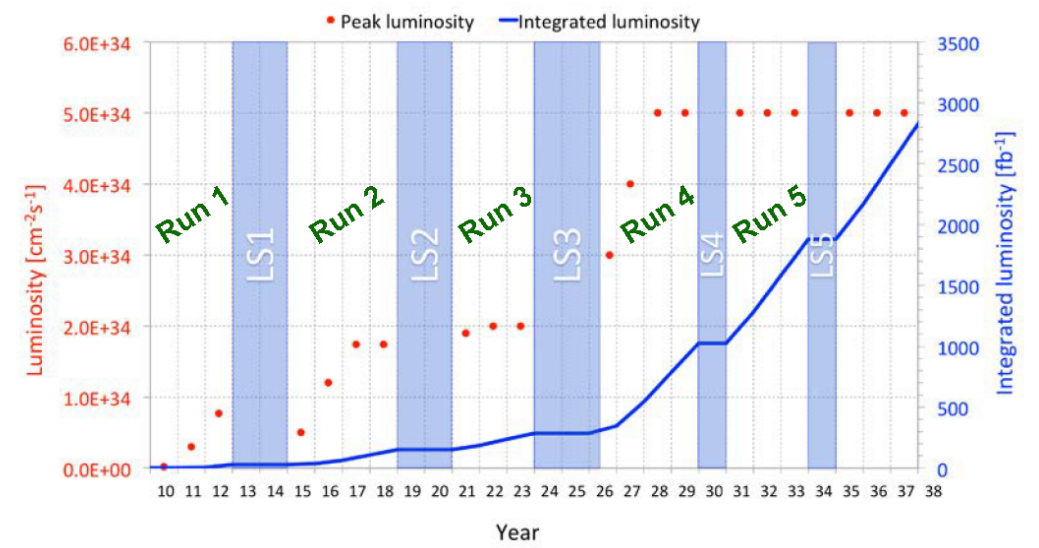
\includegraphics[width=\plotwidth]{fig/chapt3/HL-LHC-nominal.png}\\
			\caption{\label{fig:HL-LHC-Timeline:A}}
		\end{subfigure}
		\begin{subfigure}{\linewidth}
			\centering
			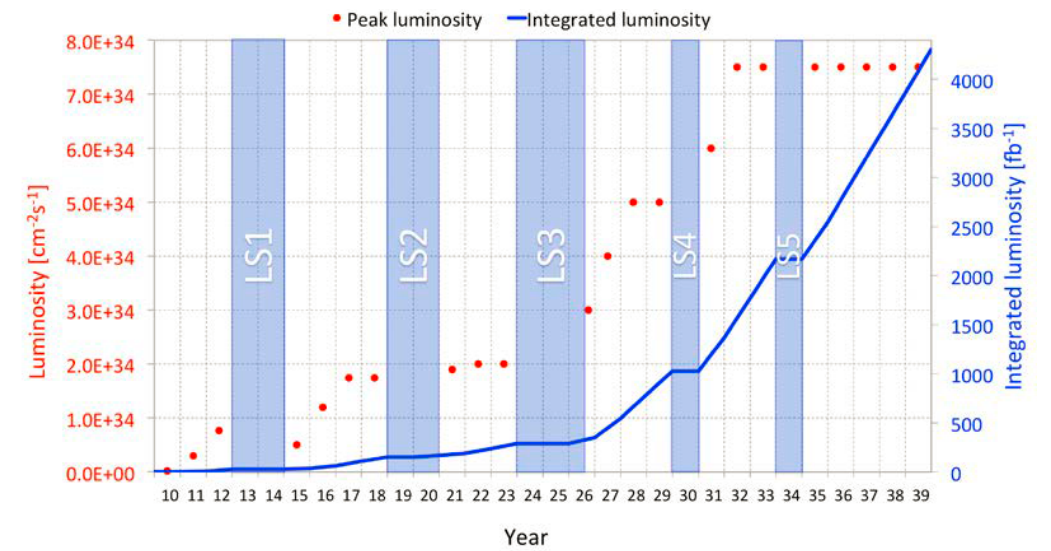
\includegraphics[width=\plotwidth]{fig/chapt3/HL-LHC-ultimate.png}
			\caption{\label{fig:HL-LHC-Timeline:B}}
		\end{subfigure}
		\caption{\label{fig:HL-LHC-Timeline} Detailed timeline projection of for LHC and HL-LHC operation until 2039 showing the evolution of the instanteneous and integrated luminosity as designed (Figure~\ref{fig:HL-LHC-Timeline:A}) and in the ultimate case where the instantaneous luminosity is increased to $7.5\times10^{34}$ \si{cm^{-2}s^{-1}} (Figure~\ref{fig:HL-LHC-Timeline:B})~\cite{HLLHC2017,HLLHCPDR}.}
	\end{figure}
		
	After approximately 15 years of operation, the LHC will undergo a new series of upgrade during the LS3 in order to boost its discovery potential as showed in Figure~\ref{fig:HL-LHC-Timeline}. This moment onward is what is referred to HL-LHC or Phase-II. The goal is to aim for a luminosity 5 to 7 times stronger than the nominal one trying to reach even 10 times this value if possible. Increasing the luminosity means that the beam size at the collision points needs to be reduced to boost the number of collisions per bunch crossing. For this purpose, new focusing and bending magnets, and collimators will be installed at the collision points as well as newly developed \textit{"crab cavities"} that will tilt the particle bunches just prior to the collisions by giving them transverse momentum and thus increasing their meeting area. In addition, the full proton injection line will be upgraded.
	
	Over its full lifetime, the HL-LHC is expected to deliver an outstanding integrated luminosity of \SI{3000}{fb^{-1}} leading, in the case of Higgs studies to measuring the couplings of the boson to a precision of 2 to 5\% thanks to the estimated 15 millions of Higgs created every year providing a more precise measurement of potential deviations from the theoretical predictions. SUSY and heavy gauge boson studies would also see their mass range limits pushed away by at least \SI{1}{TeV} and could lead to a new breakthrough. SUSY is a particularly important topic as it could give an answer to why the Higgs boson can stay so light while coupled to heavy particles by introducing the contributions of the super partners on top of providing dark matter candidates. Finally, the increase of luminosity will give the possibility to investigate "exotic" mode like for example the models introducing extra dimensions to explain the hierarchy problem.
	
	On the experiments side, the \acf{PU} will be increased up to 150 to 200 interactions per bunch crossing in ATLAS and CMS, making necessary an strong upgrade of the trigger system and of the inner trackers and of the calorimeters. Both ATLAS and CMS will also need to upgrade the muon trigger at the level of the endcaps mainly focusing on the coverage near the beam line in order to increase the detection acceptance and event selection. Moreover, the increased luminosity will also lead to an increased background rate and a faster ageing of the detectors. This PhD work takes place into this very specific context of muon detector consolidation and certification for the HL-LHC period in order to provide the CMS experiment with robust new detectors and confirm that the present system will survive through the next 20 years of HL-LHC.

	\begin{figure}[H]
		\centering
		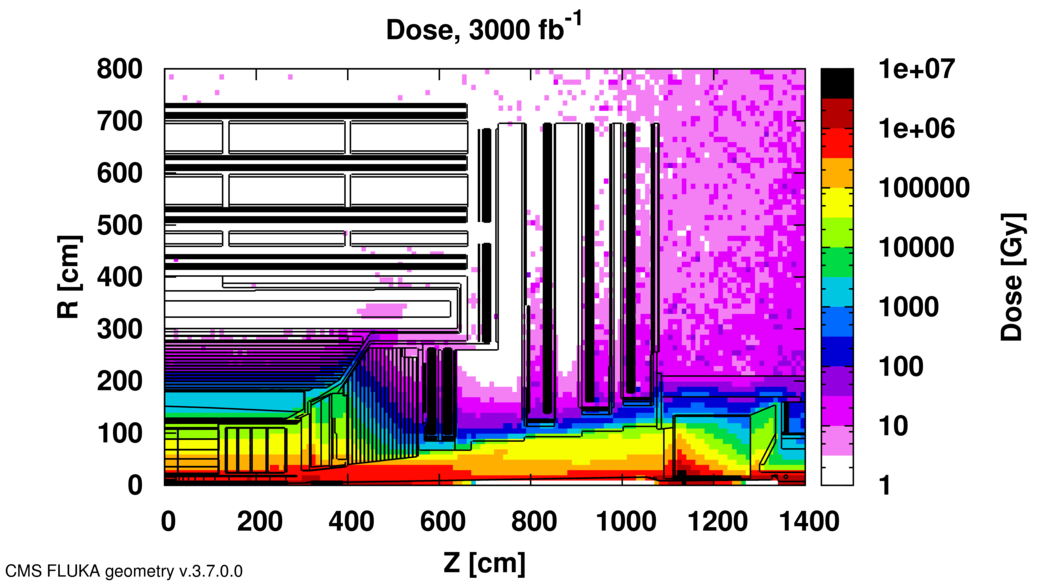
\includegraphics[width=0.7\textwidth]{fig/chapt3/HL-LHC-Dose.png}
		\caption{\label{fig:Dose} Absorbed dose in the CMS cavern after an integrated luminosity of \SI{3000}{\femto\per\barn}. Using the interaction point as reference, R is the transverse distance from the beamline and Z is the distance along the beamline.}
	\end{figure}

	The end of 2018 will mark the beginning of LS2 and the start of Phase-II upgrade activities. From the HL-LHC period onwards, i.e. past LS3, the performance degradation due to integrated radiation as well as the average number of inelastic collisions per bunch crossing, seen as pile-up into the detectors' readout that far exceeds this of the original LHC plans, will rise substantially and become a major challenge for all of the LHC experiments, like CMS, that were forced to address an upgrade program for Phase-II~\cite{PHASEIITP}. Dealing with the data from the muon detectors will force to upgrade the detectors and electronics towards the most recent technologies. Simultaneously, this will push new latency requirements onto the Level-1 trigger and the \acf{DAQ} that will only be fulfilled by upgrading the system with electronics having deeper buffering and faster processing. Simulations of the expected distribution of absorbed dose in the CMS detector under HL-LHC conditions show, in Figure~\ref{fig:Dose}, that detectors placed close to the beam line will have to withstand high irradiation, the radiation dose being of the order of a few tens of \si{Gy}.
	
	\begin{figure}[H]
		\centering
		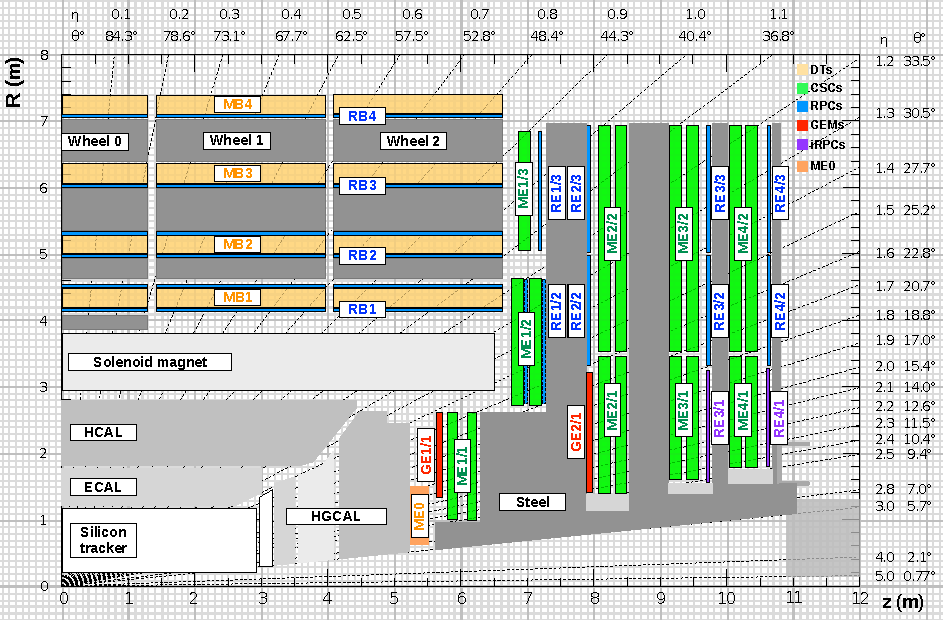
\includegraphics[width=0.7\textwidth]{fig/chapt3/Phase2_Muon_quadrant.pdf}
		\caption{\label{fig:P2Quadrant} A quadrant of the muon system, showing DTs (yellow), RPCs (blue), and CSCs (green). The locations of new forward muon detectors for Phase-II are contained within the dashed box and indicated in red for GEM stations (ME0, GE1/1, and GE2/1) and dark blue for improved RPC (iRPC) stations (RE3/1 and RE4/1).}
	\end{figure}

	The increase of irradiation close to the beam line will affect the background rate seen by the muon detectors in this area and tracking muons will prove to be difficult as this region is not yet equipped with all the detectors that were already foreseen for Phase-I. Improving this situation will come with the increase of hit numbers recorded along the particle track to reduce the ambiguity on muon versus background detection. Moreover, the measurement of small production cross-section and/or decay branching ratio processes, such as the Higgs boson coupling to charge leptons, and in particular to muons, or the $B_s \longrightarrow \mu^+\mu^-$ decay, is of major interest and specific upgrades in the forward regions of the detector will be required to maximize the physics acceptance to the largest possible solid angle.
	
To ensure proper trigger performance within the present coverage, the muon system will be completed with new chambers and the electronics of the present system will need to be upgraded to ensure an efficient triggering. Figure~\ref{fig:P2Quadrant} shows the addition of \acf{GEM} and \acf{iRPC} in the pseudo-rapidity region $1.6<\vert\eta\vert<2.4$ to complete the redundancy of the already existing CSCs as originally scheduled in the CMS Technical Proposal~\cite{CMSTP}. A first step into this direction will be taken by installing GEMs on the first endcap disk in position GE1/1 during LS2, during which preparations for the future installation of more GEMs and RPCs will take place by installing the needed services. During the YETS following LS2, iRPCs will be installed on the third and fourth endcap disks in position RE3/1 and RE4/1, and more GEMs will equip the second endcap in position GE2/1 and the inner layer, closest to the HCAL endcap called ME0 during LS3, finally completing the redundant coverage of the muon system and extending it a little by extending the reach to \psrape{2.8}, the redundancy in the region \psrapr{2.4}{2.8} being maintained by the 6 GEM layers contained in each ME0 detector that provide enough tracking points to efficiently reject neutron-induced background.
	
	Nevertheless, the region beyond \psrapg{2.8} and extending to \psrape{5.0} only is covered by the forward HCAL detectors and lack redundant muon detector coverage. Extensions of the tracker in the context of HL-LHC will increase its coverage up to \psrape{4.0} but the identification of muons and measurement of their energy with reasonable precision only using the tracker is nearly impossible. Thus, this increased tracker coverage range needs to be put in parallel with a matching muon detector and will open doors to multi-lepton final states in which leptons are likely to have a a low transverse momentum and to be found near the beam line.\\
	
	Finally, as the muon system is composed only of gaseous detectors, strong environmental concerns have risen over the last years as the European directives will restrict the use of fluorine based gas mixtures. Both the CSC and RPC subsystems, using $CF_4$, $C_2H_2F_4$, or $SF_6$, will need to adapt their working gas in order to strongly reduce the greenhouse potential of the mixtures released into the atmosphere due to gas leaks.
	
\section{Necessity for improved electronics}
\label{chapt3:sec:electronics}

	Drift Tubes and Cathode Strip Chambers are important components used to identify and measure muons, especially thanks to their spatial resolution of the order of \SI{100}{\micro m}. Nevertheless, the luminosity and irradiation during HL-LHC will cause serious event loss and ageing on the electronics of these subsystems that will comprise the triggering and data transfering needs of CMS. Thus, electronics upgrade are foreseen to address these expected problems. While only the RPCs' electronic system is able to operate under Phase-II requirements, DTs and CSCs will need to improve their trigger accept rate and latency to ensure that Level-1 trigger threshold stays at the same level~\cite{LEVEL1IR}, and DAQ data transfer rate, that respectively need to achieve a minimum of \SI{500}{kHz}, get down to \SI{12.5}{\micro s}~\cite{CMSIITP}, and increase to \SI{1082}{Gbit/s} DTs and to \SI{1026}{Gbit/s} for CSCs. As of today, the Level-1 trigger accept rate of DTs doesn't reach \SI{300}{kHz} while this of CSCs is bellow \SI{250}{kHz} but the foreseen upgrades are expected to increase the rate way beyond the requirement in the of DTs and up to \SI{4}{MHz} for CSCs~\cite{PHASEIITP}.
	
	The \acf{MiC1} used by DTs don't allow for high enough trigger rate. In addition to this problem, it was showed that these electronics contain components that are not radiation hard enough to sustain HL-LHC conditions and thus, a too large number of channels may fail due to radiations. Considering the most optimistic scenario, at least 19\% of the channels could have failed by LS4, as explicited in Figure~\ref{fig:DT-upgrade}, far before the end of the HL-LHC campain. The MiC1 will be replaced on each detector by an improved version referred to as MiC2 while front-end electronics and high-voltage modules will not need any replacement. On the other hand, CSCs showed that there electronics would be able to live through the 10 years of Phase-II but the limited buffer depth might cause memory overflows and readout inefficiencies with a fraction of event loss ranging from 5 to more than 10\% at an instantaneous luminosity similar to which of HL-LHC depending on the expected background, as showed on Figure~\ref{fig:CSC-upgrade} through the different detector positions. Thus the replacement of CSCs' \acf{CFEBs} by digital ones, DCFEBs, with deeper buffer would permit to make event loss negligible and satisfy HL-LHC requirements~\cite{PHASEIITP}.
	
	\begin{figure}[H]
		\begin{subfigure}{\linewidth}
			\centering
			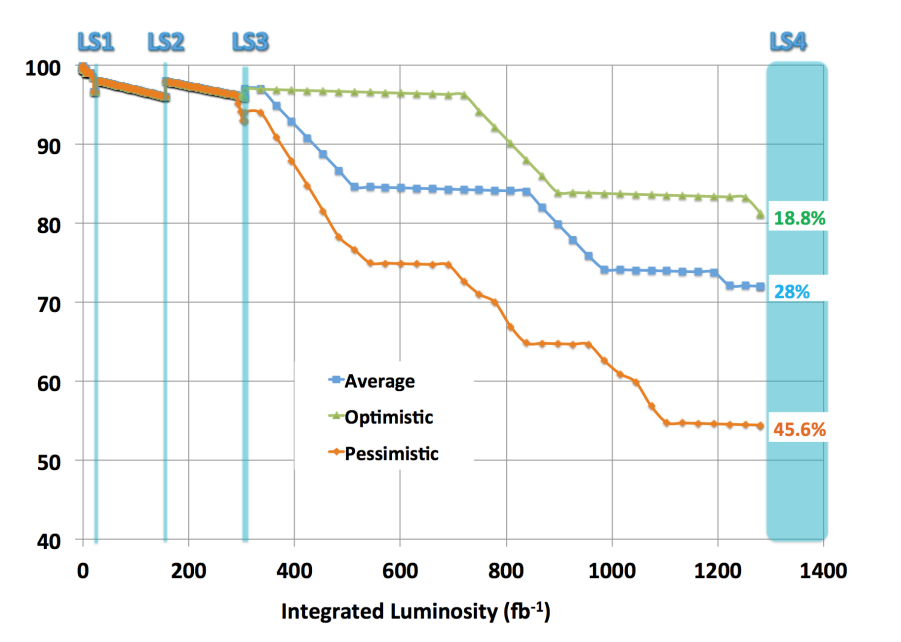
\includegraphics[width=0.8\plotwidth]{fig/chapt3/DT-channel-failure.png}\\
			\caption{\label{fig:DT-upgrade:A}}
			
		\end{subfigure}
		\begin{subfigure}{\linewidth}
			\centering
			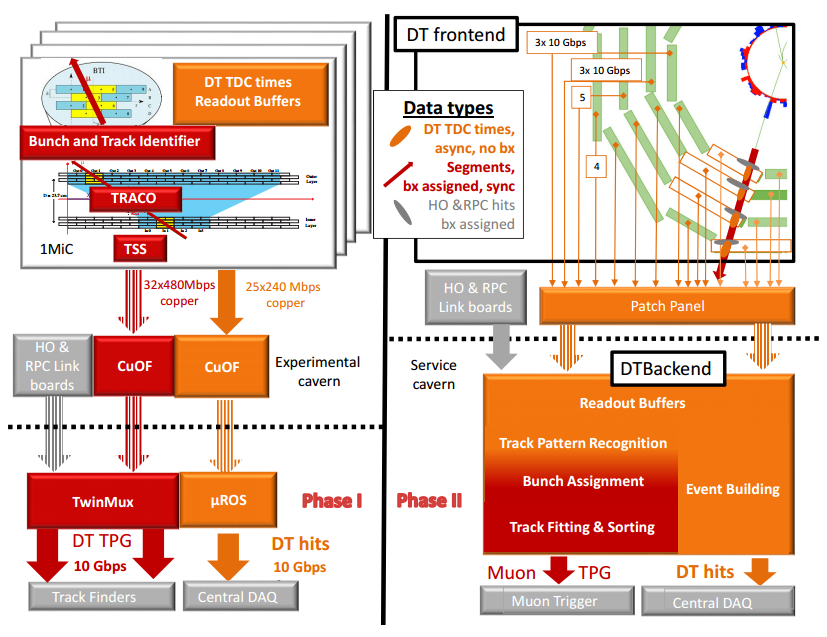
\includegraphics[width=0.9\plotwidth]{fig/chapt3/DT-upgrade.png}
			\caption{\label{fig:DT-upgrade:B}}
		\end{subfigure}
		\caption{\label{fig:DT-upgrade} Figure~\ref{fig:DT-upgrade:A}: Extrapolated fraction of failing channels of the present DT MiC1 electronics as a function of the integrated luminosity for different scenari until LS4. Figure~\ref{fig:DT-upgrade:B}: Comparison of the current (left) and upgraded (right) DT data processing. So far, the data is sent to service cavern of CMS facility via copper-to-optical-fiber translators (CuOF) by each MiC1. There, data including RPCs and outer hadron calorimeter is combined into trigger primitives (TPG) and transmitted by the TwinMux system to CMS Track Finder. The time-to-digital converter (TDC) data is collected and sent to the CMS data acquisition system (DAQ) by the micro read-out server ($\mu$ROS). After the upgrade, the TDC data will be sent via optical links to a patch panel inside the experimental cavern by each MiC2, and transferred to the back-end, where triggering and event building will be performed.}
	\end{figure}
	
	\begin{figure}[H]
		\begin{subfigure}{\linewidth}
			\centering
			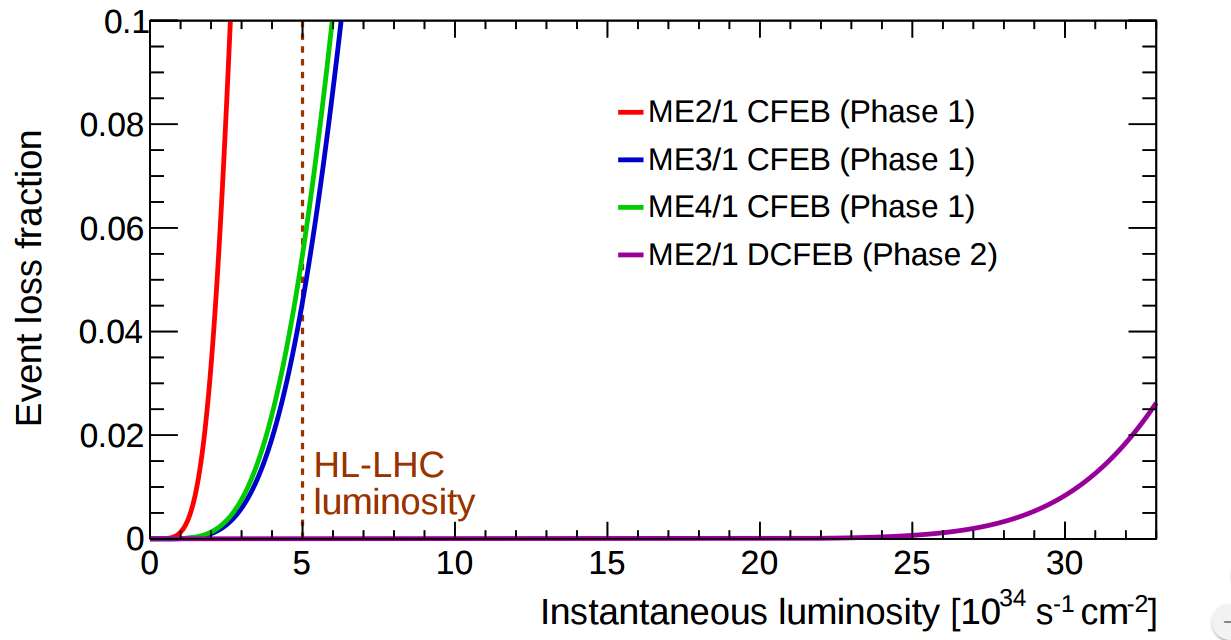
\includegraphics[width=\plotwidth]{fig/chapt3/CSC-event-loss.png}\\
			\caption{\label{fig:CSC-upgrade:A}}
		\end{subfigure}
		\begin{subfigure}{\linewidth}
			\centering
			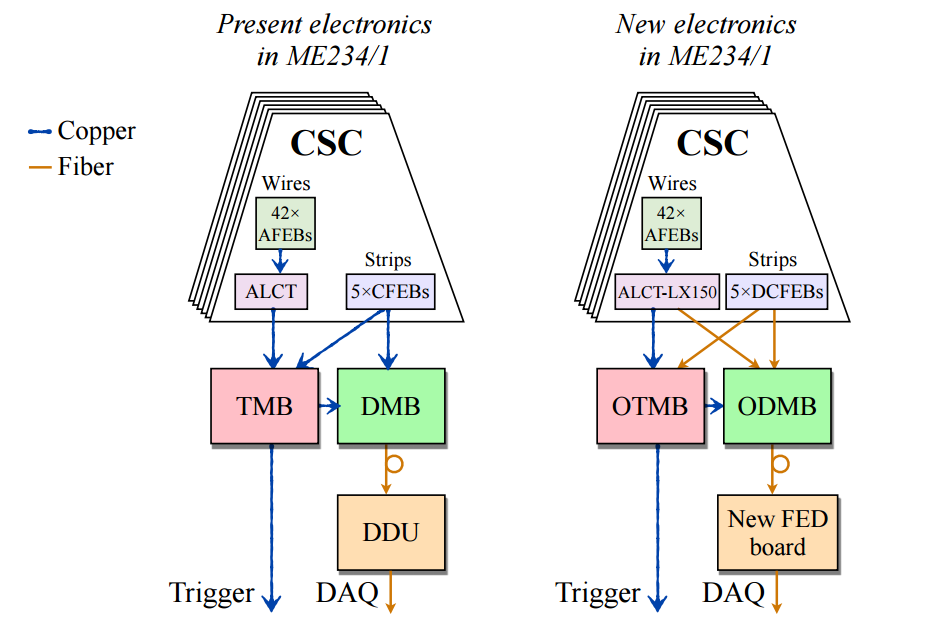
\includegraphics[width=\plotwidth]{fig/chapt3/CSC-upgrade.png}
			\caption{\label{fig:CSC-upgrade:B}}
		\end{subfigure}
		\caption{\label{fig:CSC-upgrade} Figure~\ref{fig:CSC-upgrade:A}: The event loss fractions as a function of the instantaneous luminosity is compared for CFEBs (Phase-1) and DCFEBs (Phase-II) at different CSC locations. HL-LHC luminosity is marked with the dashed brown line. Figure~\ref{fig:CSC-upgrade:B}: Comparison of the current (left) and upgraded (right) CSC data processing. A part of the connections in between ALCTs and DCFEBs, and the trigger mother boards (TMBs) and data acquisition mother boards (DMBs) will be upgraded toward optical data transfer. The detector dependent units (DDUs) used as interface in betweend CSCs' front-end electronics and the CMS DAQ will be replaced by new FED boards.}
	\end{figure}
	
	All these new DT and CSC electronics will be connected to the trigger electronics via optical links to ensure a faster communication. The main change will come from the new DT minicrate modules which will not anymore be responsible for trigger and event building logic which will be transfered to the back-end electronics instead located in the service cavern via the patch pannels to which the \acf{TDC} data will be sent. The trigger and data transfer logic will barely change for CSCs. The existing copper cable connections of cathode and anode FEBs (CFEBs, and AFEBs which data is transmitted through the ALCTs) toward the trigger and data mother boards (TMBs and DMBs) will simply be replaced by optical fibers and the TMBs and DMBs upgraded with optical versions (OTMBS and ODMBs). As a new feature, the full anode wire data from ALCTs will be sent to the ODMBs causing a lack of FPGA memory resources in these ALCT boards that will thus need replacement.
	
	\begin{figure}[H]
		\centering
		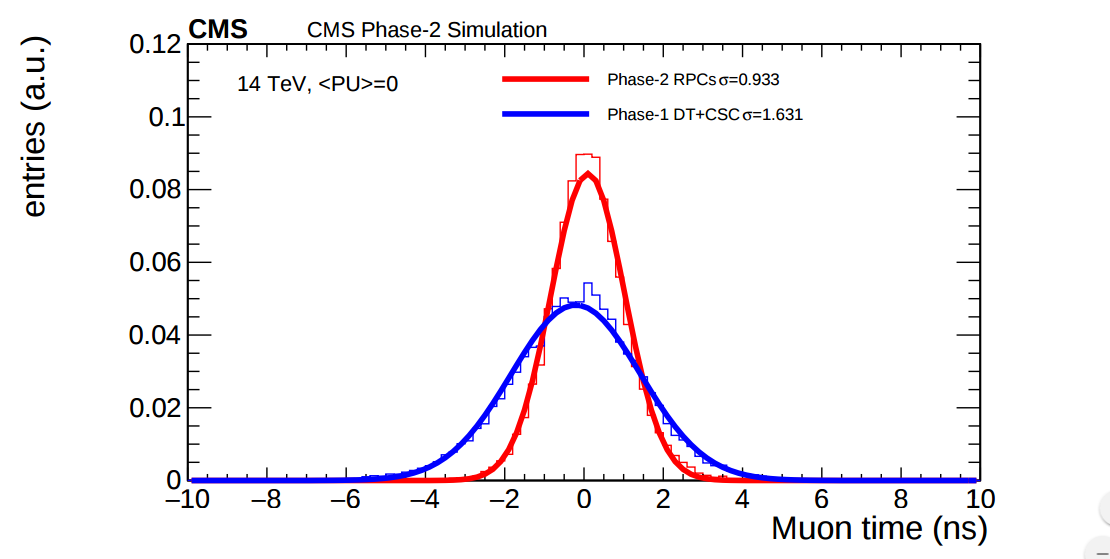
\includegraphics[width=\plotwidth]{fig/chapt3/RPC-ugrade-LS.png}
		\caption{\label{fig:RPC-time} Comparison of the simulated time residuals in between reconstructed and true muon times without (blue) and with (red) the upgraded RPC link system.}
	\end{figure}
	
	The upgrade on the side of Resistive Plate Chambers will then not come from their on-board electronics but from the Link System located in the service cavern of CMS and that connects the front-end electronics data of RPCs into CMS trigger processors. The main motivation for such and upgrade is that the electronic board composing the link system are built using obsolete components and weak components that can easily suffer from the electromagnetic noise. These components may be the source of failing channels throughout Phase-II. Moreover, these link boards were originally designed only to match RPC digitized signals with the corresponding bunch crossing. Due to this feature, the time resolution of the full RPC chain is thus limited to \SI{25}{ns} and does not exploit the full time resolution of the detectors. This would make the synchronization of the RPC system easier and allow to have a finer offline background removal within the \SI{25}{ns} in between bunch crossings thanks to the order of magnitude gained in terms of time resolution.
	
	Upgrading RPC link system will require the installation of 1376 new link boards and 216 control boards. The new boards will make use of the recent progress made with fast FPGAs and will be a great improvement to the ASICs formerly used as they will be able to process signals from several detectors in parallel. The benefice from using the full RPC time resolution thanks to the upgraded link system can be seen through Figure~\ref{fig:RPC-time} where the resolution of the RPC system itself is better than which of DTs and CSCs that was used until now.

\section{New detectors and increased acceptance}
\label{chapt3:sec:GEMRPC}

	In the present muon system, the redundancy of was assured by RPCs used for their good timing performances. The extension of the muon system towards higher pseudo-rapidity in order to complete the redundancy in this very region and to contribute to the precision of muon momentum measurements will require muon chambers with a spatial resolution less or comparable to the contribution  muon of multiple scattering through the detector volume~\cite{MUONTDR}. Most of the plausible physics is covered only considering muons with $p_T<$\SI{100}{GeV} thus, in order to match CMS requirements, a spatial resolution of $\mathcal{O}$(few $\mathrm{mm}$) will be necessary for the proposed new RPC stations while the GEMs will need a resolution better than \SI{1}{mm}, as showed by the simulation in Figure~\ref{fig:MultiScat}.

	\begin{figure}[H]
		\centering
		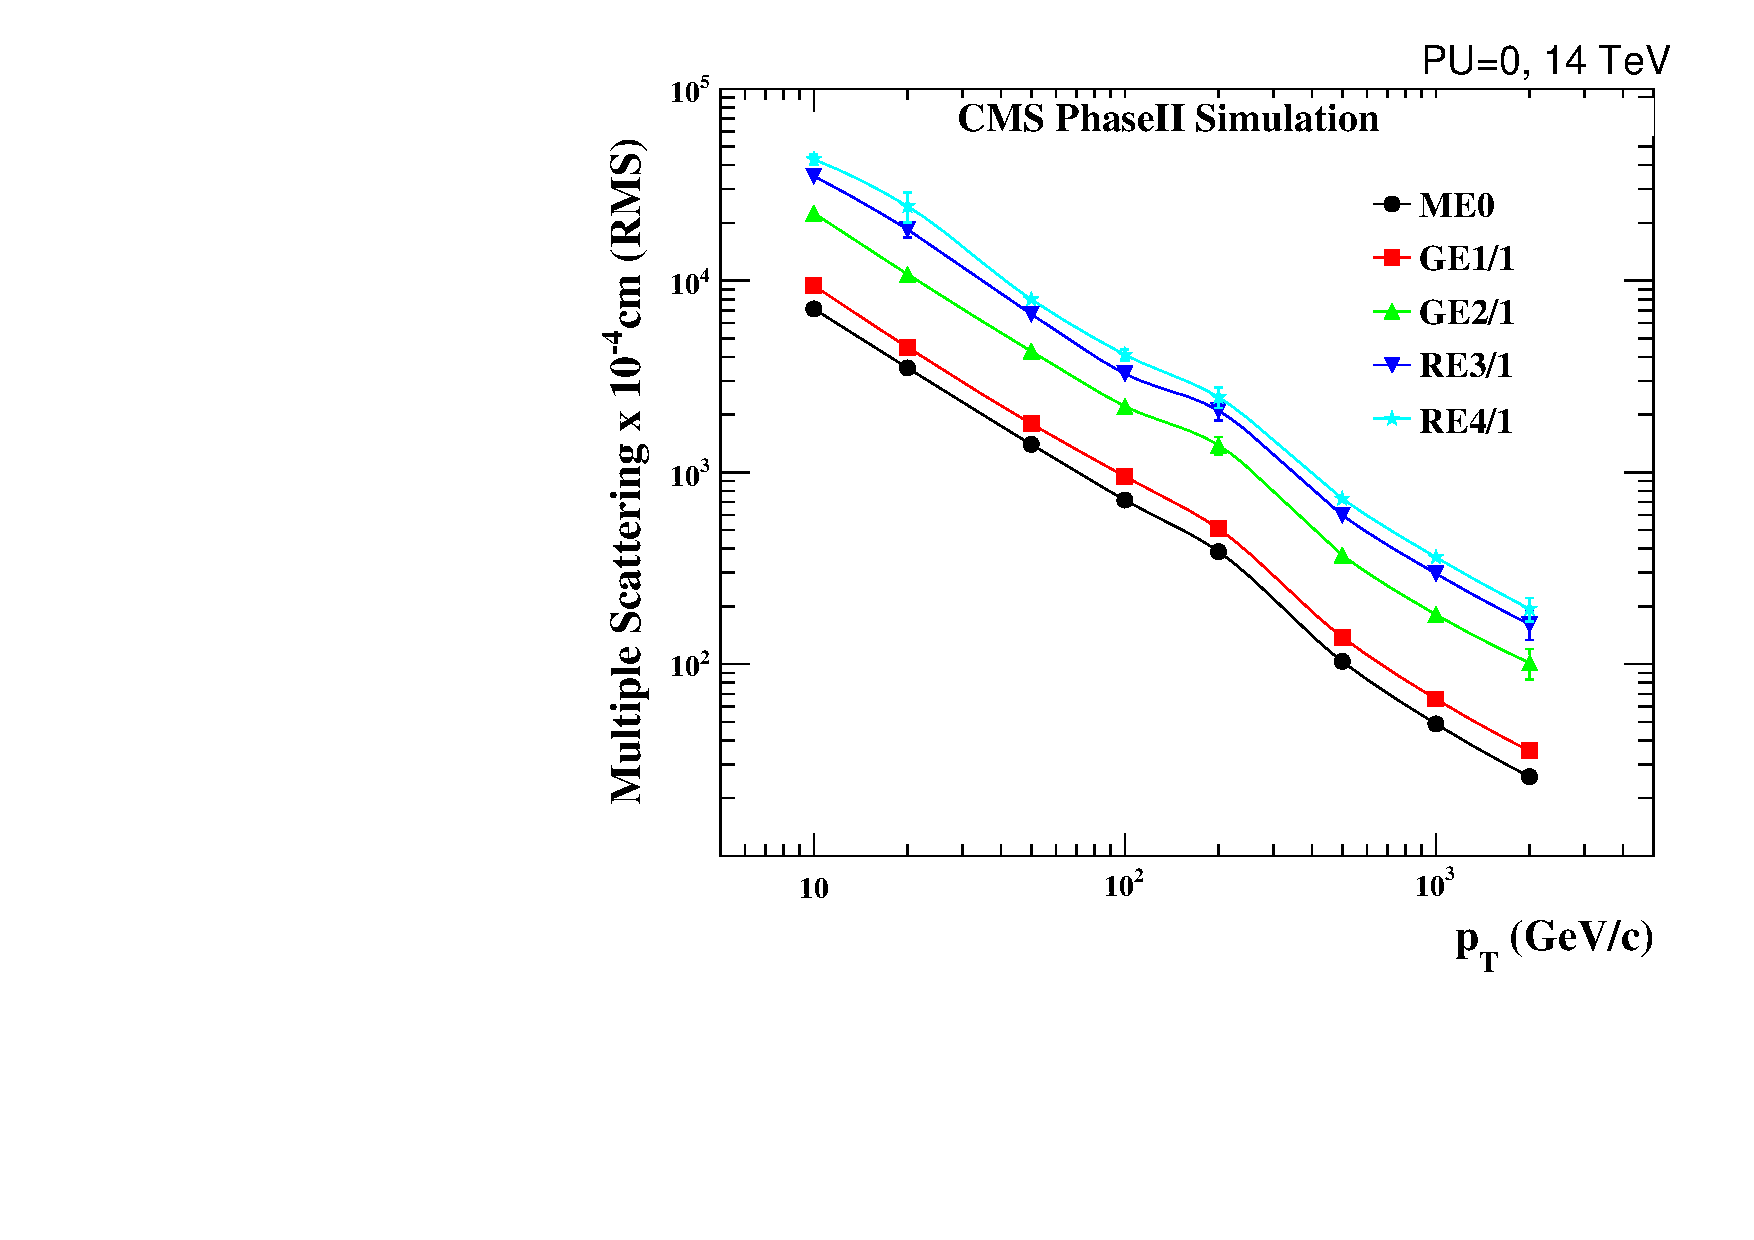
\includegraphics[width=0.6\textwidth]{fig/chapt3/MS_allstations.pdf}
		\caption{\label{fig:MultiScat} RMS of the multiple scattering displacement as a function of muon $p_T$ for the proposed forward muon stations. All of the electromagnetic processes such as bremsstrahlung and magnetic field effect are included in the simulation.}
	\end{figure}
	
	\subsection{Improved forward resistive plate chambers}
	\label{chapt3:ssec:iRPCs}

	\begin{figure}[H]
		\centering
		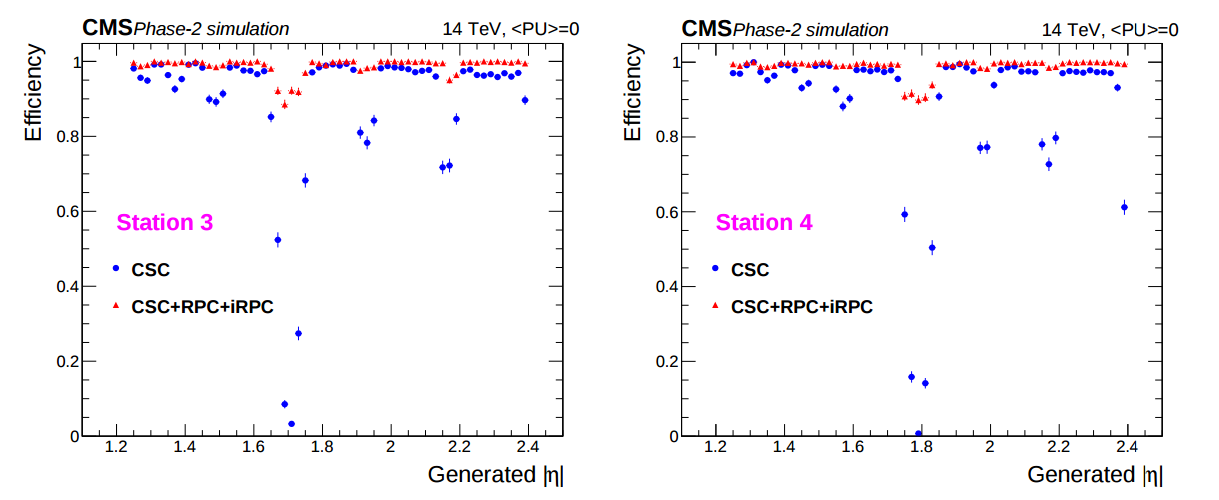
\includegraphics[width=\linewidth]{fig/chapt3/Trigger-efficiency-endcap.png}
		\caption{\label{fig:Endcap-trigger-eff} Simulation of the impact of RPC hit inclusion onto the local trigger primitive efficiency in station 3 (left) and station 4 (right). The contribution of iRPC starts above \psrape{1.8}.}
	\end{figure}
	
	Figure~\ref{fig:P2Quadrant} shows that the iRPCs that will equip the third and fourth endcap disks in position RE3/1 and RE4/1 will finally be the partners of the CSCs in position ME3/1 and ME4/1 and complete Phase-I plans but bringing the needed upgrades in the scope of Phase-II as the older chambers are not suitable to equip the forward region of CMS due to HL-LHC rates and charge deposition. By completing the redundancy, more track along the muon trajectory will be available and the lever arm will be improved. The benefits from extending the redundancy of the muon system with iRPCs to the forward most region is showed in Figure~\ref{fig:Endcap-trigger-eff} in which the trigger efficiency is showed with and without RPCs in which it is possible to see that the efficiency of CMS trigger with the complete redundancy is improved is above 95\% in the region \psrapg{1.8} as the iRPCs help filling the holes in the CSC system.\\
	
	The detectors that will be installed in the coming years will be similar to the already existing RPC system. 18 of the new chambers, each spanning \SI{20}{\degree} in $\varphi$ around the beam axis with 96 radially oriented trapezoidal read-out strips, will cover each muon endcap disk leading to the production of 72 iRPCs.The main difference with the old RPC chambers is that these detectors will not have readout strips segmented in $\eta$ as by using fast front-end electronics the strips will be read-out on both sides allowing for a radial spatial resolution of the order of \SI{2}{cm} in order to contribute to the better reconstruction of muon in the forward region where the bending of muons by the magnetic field is low. This is motivated by the fact that, in the case a $\eta$ segmentation was used, at least 5 pseudorapidity partitions would have been necessary to reach the minimal radial spatial resolution ($\approx$ \SI{20}{cm}). Having only one strip read-out from both along the chamber reduces by 60\% the total number of channels and the necessary cabling and allows for a better spatial resolution. The strip pitch will range from \SI{6.0}{mm} (\SI{5.9}{mm}) on the high pseudo-rapidity end to \SI{12.3}{mm} (\SI{10.9}{mm}) on the low one on position RE3/1 (RE4/1). The spatial resolution in the direction perpendicular to the strips should reach approximately \SI{3}{mm}, better than the minimal needed resolution (Figure~\ref{fig:MultiScat}), and the overall time resolution of the new installation will be equally \SI{1.5}{ns}, as for the present due to the same link system being used.

	\begin{figure}[H]
		\centering
		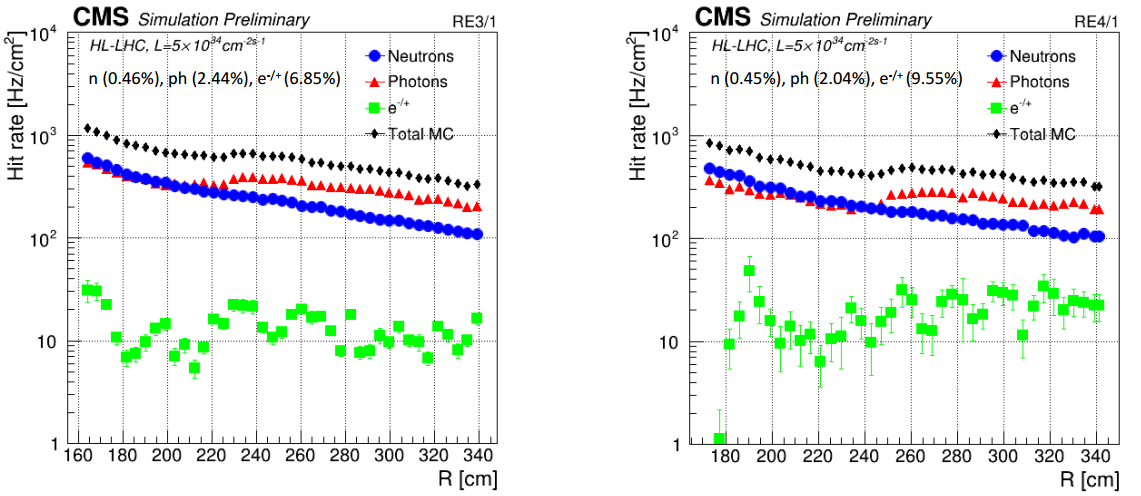
\includegraphics[width=0.6\textwidth]{fig/chapt3/RPC-Sim-HL-LHC_Rate.png}
		\caption{\label{fig:iRPC-Rate} Expected hit rate due to neutrons, photons, electrons and positrons at HL-HLC instantaneous luminosity of $5\times10^{34}$ \si{cm^{-2}s^{-1}} in RE3/1 chambers covering the region \SI{1527}{mm} $<R<$ \SI{3192}{mm}. In the upper part of the figure the sensitivities of RPCs used in the simulation for each particle are reported. The hit rates are expected to be similar in RE4/1 covering the region \SI{1770}{mm} $<R<$ \SI{3140}{mm}.}
	\end{figure}
	
	Nevertheless, having only a single strip instead of pseudo-rapidity segmentation will increase the probability of double hits in the same channel. This probability was estimated to be low enough as it shouldn't exceed 0.6\%. This estimation was made assuming an average hit rate per unit area of \SI{500}{Hz/cm^2} in the iRPCs (see Figure~\ref{fig:iRPC-Rate}), a cluster size (average number of strips fired per muon) of 2, a strip active area of \SIsurface{158.4}{0.87}{cm} and a safety factor 3 leading to an estimated rate per strip of \SI{380}{kHz} corresponding to an average time interval of \SI{2600}{ns} in between 2 consecutive hits. The time for a signal to go through the full strip length is about \SI{10}{ns} to which can be added \SI{1}{ns} of dead time and 2 TDC clock cycles of \SI{2.5}{ns} for a minimal time interval of \SI{16}{ns} necessary to avoid ambiguities. The probability of having ambiguous double hits in a strip in then the ratio in between this minimal time interval in between 2 consecutive hits and the average time interval estimated from the rate the detectors are subjected to.
	
	The instantaneous luminosity at HL-LHC being very high, the rates at the level of the new chambers needed to be simulated in order to understand the necessary requirements for these detectors. The simulated results for different background components (neutrons, photons, electrons and positrons) are showed in Figure~\ref{fig:iRPC-Rate} assuming known sensitivities to these particles. It is showed that in the hottest area, the rates could increase beyond \SI{700}{Hz/cm^2}. Thus, taking into account a safety factor of about 3, it was decided that improved RPCs should at least be certified for rates reaching \SI{2}{kHz/cm^2} which would be achieved thanks to several improvements on the design and on the electronics. The detectors design will be based on the existing RPC design as they will be double gaps. Similarly to the existing RPC system, the electrode material will be HPL although the thickness of the electrodes and of the gas gap will be reduced to \SI{1.4}{mm} as a thinner gas gap leads to a decrease of deposited charge per avalanche as showed in Figure~\ref{fig:charge-gap}. The smaller the gas gap, the more the detector becomes sensitive to gap non-uniformities across the electrode planes making a gap of \SI{1.4}{mm} a good compromise in between these two competing factors.

	\begin{figure}[H]
		\centering
		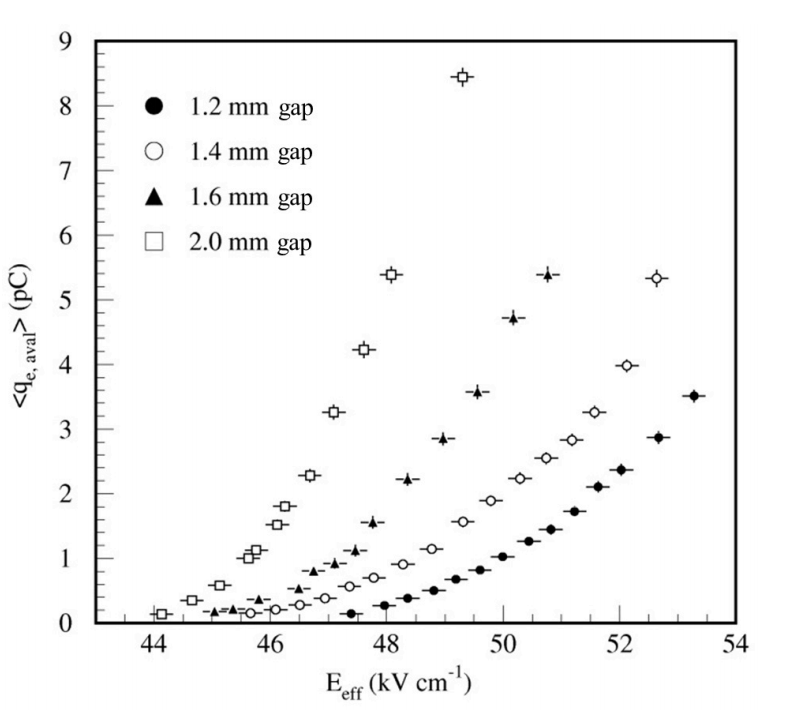
\includegraphics[width=0.8\plotwidth]{fig/chapt3/charge-vs-gap.png}
		\caption{\label{fig:charge-gap} Measured average charge per avalanche as a function of the effective electric field for different gas gap thickness in double gap RPCs using HPL electrodes.}
	\end{figure}

	\begin{figure}[H]
		\centering
		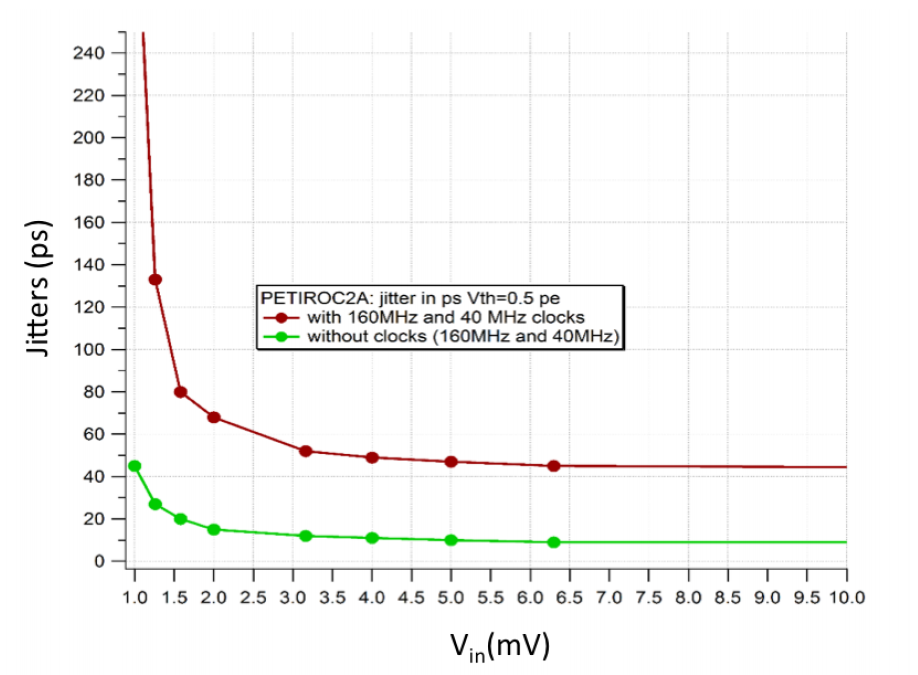
\includegraphics[width=0.8\plotwidth]{fig/chapt3/jitter-PETIROC.png}
		\caption{\label{fig:jitter} The PETIROC time jitter as a function of the input signal amplitude, measured with and without internal clocks.}
	\end{figure}
	
	A lower charge deposition inside of the detector volume means a slower ageing and a longer lifetime for detectors subjected to high irradiation. But, in order to take advantage of the lower detector gain, more sensitive electronics are required so that the part of gain that was formerly done in the gas volume can be moved to the electronics. Achieving this with the technology developed more than 10 years ago for the present system is not possible as the signal over noise ratio of such electronics doesn't allow to detect charges as low as \SI{10}{fC}. Moreover, the new front-end electronics will need to be radiation hard to survive to more than 10 years of HL-LHC conditions. The new technology that has been chosen is based on the PETIROC ASIC manufactured by OMEGA and is a 64-channel ASIC called CMS RPCROC on which the original SiGe technology will be replaced by CMOS to increase its radiation hardness while keeping fast pre-amplification and discrimination with a very low jitter that can reach less than \SI{20}{ps} if no internal clock is used, as can be seen from Figure~\ref{fig:jitter}. The ASIC is associated with an FPGA which purpose is to measure time thanks to a TDC with a time resolution of 50-100 \si{ps} developed by Tsinghua University and that will provide a measurement of the signal position along the strip with a precision of a few \si{cm} by measuring the signal timing on both ends of the strips. In order to read-out all 96 strips, 3 ASICs and 3 TDCs, each having 64 channels, are hosted on a front-end board attached to the chamber.\\
	
	{\color{blue}[Wait for the analysis of 2018 GIF++ data to add interesting information about the time and spatial resoltution measured during test beam periods.]\\}
	
	\subsection{Gas electron multipliers}
	\label{chapt3:ssec:GEMs}
	
	In the region closer to the interaction point where the spatial resolution is requested to be better than \SI{1}{mm} for the new detectors (at least for GE1/1 and ME0, GE2/1 being in the same order of requested spatial resolution than the new iRPCs that will equip the third and fourth endcaps), the choice has been made to use triple GEMs, micro pattern gaseous detectors, in the place of RPCs. The GE1/1 project had been the first to be approved and demonstrators had been installed in CMS already during LS1. The rest of the detectors will be installed during LS2 while the GE2/1 and ME0 projects are still under development. ME0, GE1/1 and GE2/1 will be installed respectively next to the HCAL endcap, on the first and on the second muon endcap disks as can be seen from Figure~\ref{fig:P2Quadrant}.

	\begin{figure}[H]
		\centering
		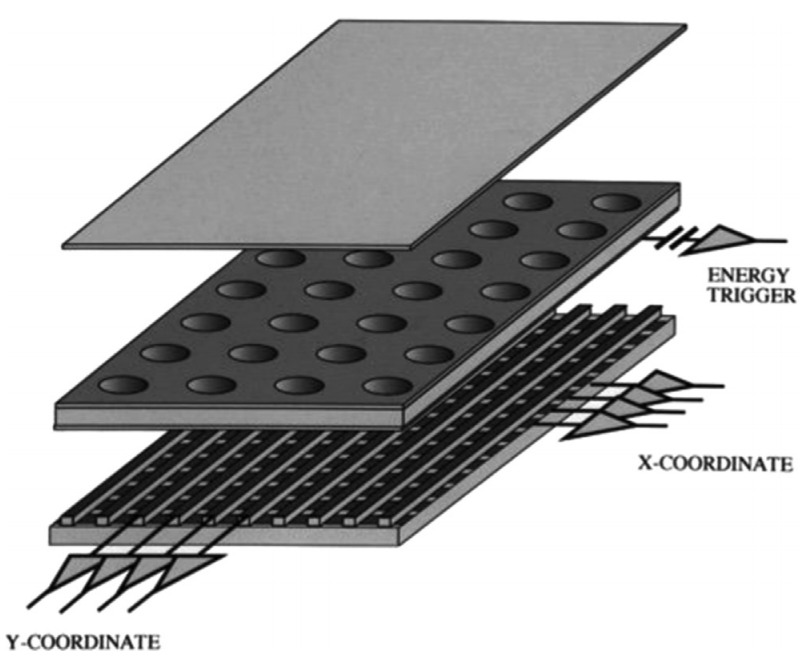
\includegraphics[width=0.7\plotwidth]{fig/chapt3/GEM.png}
		\caption{\label{fig:GEM} Schematics of a GEM showing the cathode on top, the GEM foil separating the gas volume into the drift region, in between the cathode and foil, and the induction region, in between the GEM foil and the anode, and the anode on which a 2D read-out is installed. A negative voltage is applied on the cathode while the anode is connected to the ground.}
	\end{figure}
	
	Gas Electron multipliers are gaseous detectors~\cite{SAULI97} which gas volume is confined in between 2 planar electrodes, the anode serving as read-out panel. The gas volume is divided in 2 or more regions by a single or multiple \textit{GEM foils} as showed in Figure~\ref{fig:GEM}. These foils are very thin, of the order of a few tens of \si{\micro m}, and are pierced with holes as can be seen in Figure~\ref{fig:GEM-foil}. Both surfaces of the GEM foils are clad with copper in order to apply a strong electric field in between each side that will generate very strong potentials in the holes. The gas region contained in between the cathode and the GEM foil is called the drift region as the electric field is not strong enough to cause avalanches and thus start an amplification. The primary electrons drift toward the foil and are accelerated and amplify by the very high potential within the holes, as showed in Figure~\ref{fig:GEM-foil}. Then the electrons reach the second drift region in which they will induce signal on the read-out located on the anode. By restraining the amplification process at the level of the holes, the electrons can stay in a very confined space and thus induce a very localized current, providing the GEMs with a very good spatial resolution.
	
	In order to achieve a stronger amplification, the amplification process can be repeated several times in a row. The GEMs that will be used in CMS are triple GEM detectors operated with a 70/30 gas mixture of $Ar$/$CO_2$. They contain 3 GEM foils and thus 3 electron amplifications, as can be seen in Figure~\ref{fig:GEM-drift}. The GEM foils used in CMS are \SI{50}{\micro m} foils clad with \SI{5}{\micro m} of copper on each side. The foils are pierced with double-canonical holes which inner and outer diameters are respectively 50 and \SI{70}{\micro m} which are placed \SI{140}{\micro m} from each other in an hexagonal pattern, as showed in Figure~\ref{fig:GEM-foil}. These detectors have a time resolution better than \SI{10}{ns} and reach very good spatial resolutions of less than \SI{300}{\micro m} with an angular precision of less than \SI{200}{\micro rad}.

	\begin{figure}[H]
		\centering
		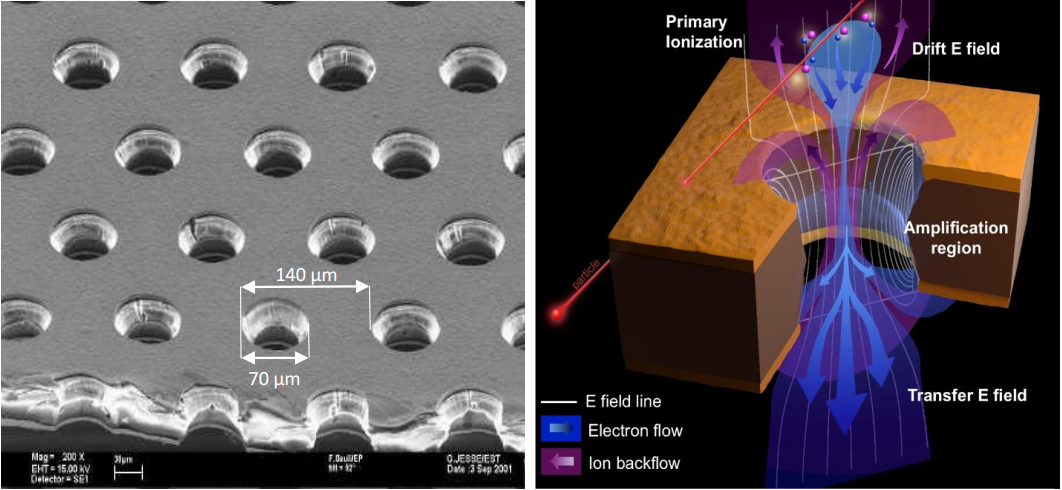
\includegraphics[width=\plotwidth]{fig/chapt3/GEM-foil-ampli.png}
		\caption{\label{fig:GEM-foil} Left: Picture of a CMS GEM foil provided by a scanning electron microscope. Righ: Representation of the electric field lines in a GEM hole and of the amplification that electrons and ions undergo in the hole's volume due to the very intense electric field.}
	\end{figure}

	\begin{figure}[H]
		\centering
		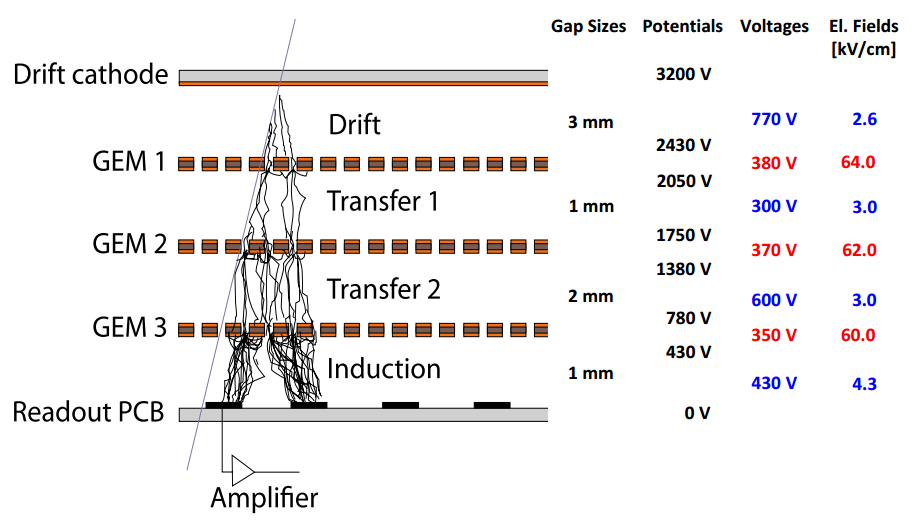
\includegraphics[width=\plotwidth]{fig/chapt3/GEM-drift.png}
		\caption{\label{fig:GEM-drift} Schematic representation of CMS triple GEMs. The gas volume is divided into 4 areas. The drift area is the region where the primary electrons are created before being amplified a first time while passing through the first GEM foil. Then the process of drift and amplification is repeated twice in following two transfer areas and GEM foils. Finally, the charges have been amplified enough to induce current in the read-out strips while in the last drift area. The dimensions, potentials and electric fields are provided.}
	\end{figure}
	
	The GEM Upgrade is divided into 3 subsystems as GE1/1 was the first approved project~\cite{GEM11TDR} and that the detectors will already be installed during LS2. GE2/1 and ME0, on the other hand, will profit of the R\&D knowledge and skills developed for GE1/1 while the requirements for each subsystem are different as they are not placed at the same distance from the interaction point. In this very forward region, a different position with respect to the center of the detector can change dramatically the conditions in which the detectors will have to be operated. In terms of rate capability, GE2/1, which is the furthest, is required to whisthand \SI{2.1}{kHz/cm^2} while GE1/1 needs to be better than \SI{10}{kHz/cm^2} and ME), better than \SI{150}{kHz/cm^2}. In terms of ageing with respect to charge deposition, ME0 needs to be certified to \SI{840}{mC/cm^2}, GE1/1 to \SI{200}{mC/cm^2} and GE2/1 only to \SI{9}{mC/cm^2}. All 3 detectors need to have a time resoltion better than \SI{10}{ns} and an angular resolution better than \SI{500}{\micro rad}.
	
	Adding the GEMs into the forward region of the muon system will allow to strongly enhance the Level-1 Trigger performance by reducing the inefficiency regions and the trigger rate as showed in Figure~\ref{fig:GEM-Trigger}. Moreover, benefiting from the good spatial and angular resolution of the GEMs, the precision into the muon measurement will also be greatly improved by the addition of GEMs as can be seen from the simulation presented in Figure~\ref{fig:GEM-Muon}.

	\begin{figure}[H]
		\centering
		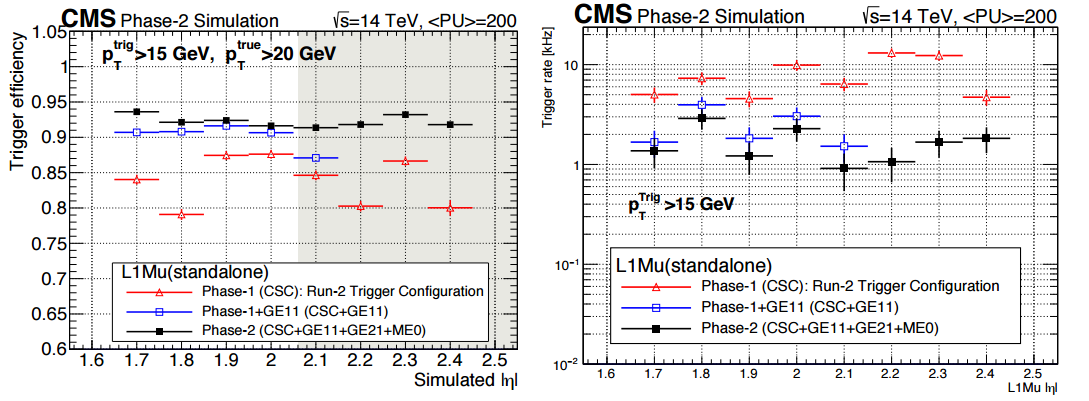
\includegraphics[width=\linewidth]{fig/chapt3/GEM-Trigger.png}
		\caption{\label{fig:GEM-Trigger} Simulated efficiency and rate of the standalone Level-1 muon trigger using tracks reconstructed in CSCs and all GEM stations compared with Phase-I values in the case where only CSCs are used or CSCs+GE1/1. The zones of inefficiency of the CSC subsystem are compensated by the addition of GEMs during Phase-II and the trigger rates is kept from increasing due to the high luminosity.}
	\end{figure}
	
	\begin{figure}[H]
		\begin{subfigure}{0.6\linewidth}
			\centering
			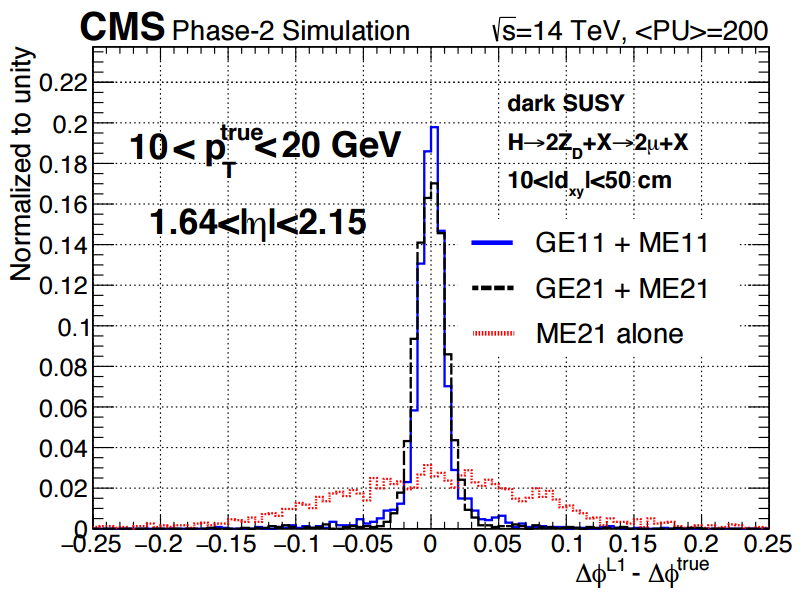
\includegraphics[height=5cm]{fig/chapt3/GEM-muon-direction.png}
			\caption{\label{fig:GEM-Muon:A}}
		\end{subfigure}
		\begin{subfigure}{0.4\linewidth}
			\centering
			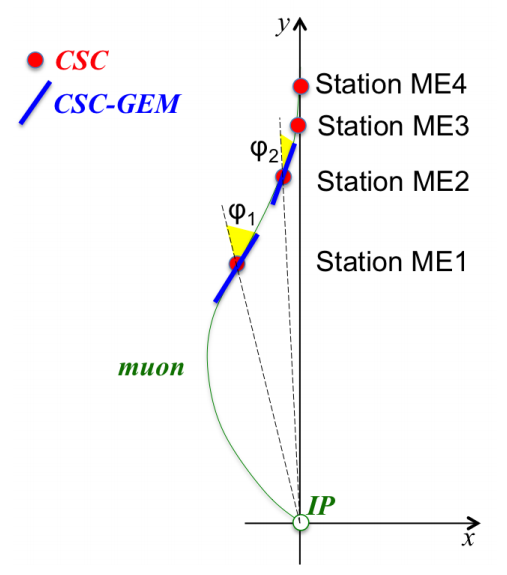
\includegraphics[height=6cm]{fig/chapt3/GEM-Muon-bending.png}
			\caption{\label{fig:GEM-Muon:B}}
		\end{subfigure}
		\caption{\label{fig:GEM-Muon} Figure~\ref{fig:GEM-Muon:A}: Simulated resolution of the muon direction measurement $\Delta\phi$ with Phase-II conditions. In the second endcap station, the resolution is compared in the case of CSCs (ME2/1) alone and CSCs+GEMs (GE2/1+ME2/1) while a similar resolution measurement is given in the case of the first station (GE1/1+ME1/1). Figure~\ref{fig:GEM-Muon:B}: The addition of GEM detectors on stations 1 and 2 (ME0 is considered to contribute to station station 1) as redundant system to CSCs allows to improve the muon momentum improvement through a more accurate measurement of the local bending angles $\phi_1$ and $\phi_2$.}
	\end{figure}
	
	\subsection{Installation schedule}
	\label{chapt3:ssec:schedule}

\section{Implications of the different upgrades on the Level-1 Trigger. Improvement of physics performance.}
\label{chapt3:sec:L1tP2}

\section{Ecofriendly gas studies}
\label{chapt3:sec:EcoGas}

	\subsection{Status of the studies and potential candidates}
	\label{chapt3:ssec:GasStatus}

	\subsection{Implications in case of no suitable ecofriendly mixture}
	\label{chapt3:ssec:GasConsequences}

\clearpage{\pagestyle{empty}\cleardoublepage}